% This file was created with tikzplotlib v0.10.1.
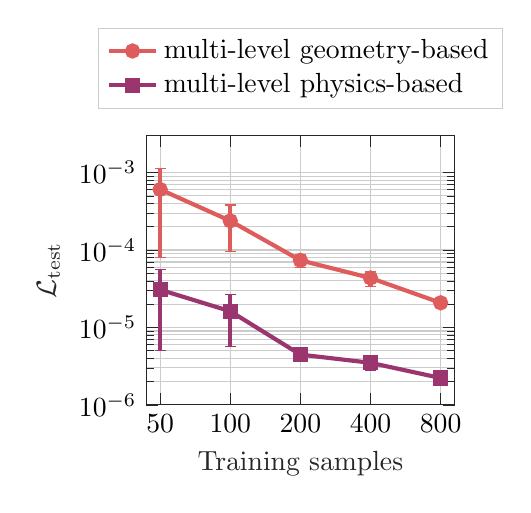
\begin{tikzpicture}

\definecolor{darkslategray38}{RGB}{38,38,38}
\definecolor{indianred2229291}{RGB}{222,92,91}
\definecolor{lightgray204}{RGB}{204,204,204}
\definecolor{mediumvioletred15453111}{RGB}{154,53,111}

\begin{axis}[
width=5.5cm,
height=5cm,
axis line style={darkslategray38},
legend cell align={left},
legend columns = 1,
legend style={
  fill opacity=1,
  draw opacity=1,
  text opacity=1,
  at={(0.5,1.1)},
  anchor=south,
  draw=lightgray204
},
    log basis x={10},
    log basis y={10},
    tick align=inside,
    x grid style={lightgray204},
    xlabel=\textcolor{darkslategray38}{Training samples},
    xmajorgrids,
    xmajorticks=true,
    xminorticks=true,
    xmin=43.5275281648062, xmax=918.958683997629,
    xmode=log,
    xtick style={color=darkslategray38},
    xtick={50,100,200,400,800},
    xticklabels={
      \(\displaystyle {50}\),
      \(\displaystyle {100}\),
      \(\displaystyle {200}\),
      \(\displaystyle {400}\),
      \(\displaystyle {800}\)
    },
    y grid style={lightgray204},
    ylabel=\textcolor{darkslategray38}{\(\displaystyle \mathcal{L}_{\mathrm{test}}\)},
    ymajorgrids,
    yminorgrids,
    ymajorticks=true,
    ymin=1e-06, ymax=0.003,
    ymode=log,
    ytick style={color=darkslategray38},
    % ytick={1e-06,1e-05,0.0001,0.001},
    % yticklabels={
    %   \(\displaystyle {10^{-6}}\),
    %   \(\displaystyle {10^{-5}}\),
    %   \(\displaystyle {10^{-4}}\),
    %   \(\displaystyle {10^{-3}}\)
    % }
]

\addplot+[line width = 1.5pt,
  indianred2229291, mark options={indianred2229291, scale=1},
  error bars/.cd, 
    y fixed,
    y dir=both, 
    y explicit,
    error bar style={line width=1.5pt}
] table [x=x, y=y,y error=error, col sep=comma] {
    x,  y,       error
    50, 0.0006057525897631422, 0.0005253575150020925
    100, 0.00023783658252796158, 0.0001428717883669156
    200, 7.355117559200152e-05, 1.4805785250195808e-05
    400, 4.349869341240265e-05, 9.808991600950175e-06
    800, 2.07822668e-05, 0
};
% \addlegendentry{GBF-B-GUN}
\addlegendentry{multi-level geometry-based}

\addplot+[line width = 1.5pt,
  mediumvioletred15453111, mark options={mediumvioletred15453111, scale=1},
  error bars/.cd, 
    y fixed,
    y dir=both, 
    y explicit,
    error bar style={line width=1.5pt}
] table [x=x, y=y,y error=error, col sep=comma] {
    x,  y,       error
    50, 3.066722019866575e-05, 2.5689228637218805e-05
    100, 1.6163716009032213e-05, 1.0445283178417746e-05
    200, 4.454451618585153e-06, 8.414642202987869e-07
    400, 3.4899384445452596e-06, 7.467996986727589e-07
    800, 2.2180977339303354e-06, 0
};
% \addlegendentry{PBF-B-GUN}
\addlegendentry{multi-level physics-based}
\end{axis}

\end{tikzpicture}

%  legend pos=south,
  % legend style={draw=none}